% --------------------------------------|
% -------------------------------------|
% ------------------------------------|
\section{Comparación de Resultados} 
% ------------------------------------\
% --------------------------------------\
% ----------------------------------------\
{\large\textbf{DFS:}}

\begin{enumerate}
    \item \textbf{Enfoque:} Backtracking, exploración profunda.
    \item \textbf{Exploración:} Se adentra tanto como sea posible antes de retroceder.
    \item \textbf{Optimización:} No garantiza encontrar la solución más corta.
    \item \textbf{Encuentra:} Una solución y muestra la ruta.
    \item \textbf{Distancia:} No considera la distancia, no hay garantía de que use la ruta más corta.
    \item \textbf{Eficiencia:} Puede ser eficiente en laberintos con caminos ramificados y no es 
    necesario encontrar la ruta más corta.
\end{enumerate}

\begin{figure}[h]
    \centering
    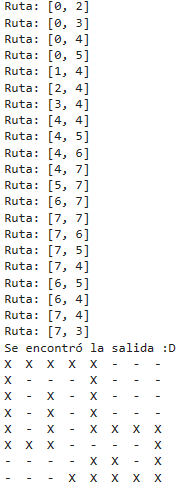
\includegraphics[scale = .6]{IMA/captuDFS.png}
    \caption{DFS}
    \label{fig:enter-label}
\end{figure}
\vspace{0.5cm}

{\large\textbf{BFS:}}

\begin{enumerate}
    \item \textbf{Enfoque:} Exploración nivel por nivel.
    \item \textbf{Exploración:} Comienza explorando todos los nodos a una 
    distancia \(d\) antes de pasar a los nodos a una distancia \(d+1\).
    \item \textbf{Optimización:} Garantiza encontrar la solución más corta. Garantiza la optimización.
    \item \textbf{Distancia:} Encuentra la ruta más corta desde el inicio hasta la salida.
    \item \textbf{Eficiencia:}Evita Explorar caminos no óptimos.
    \item \textbf{Evita:} Explorar caminos no óptimos.
\end{enumerate}

\begin{figure}[h]
    \centering
    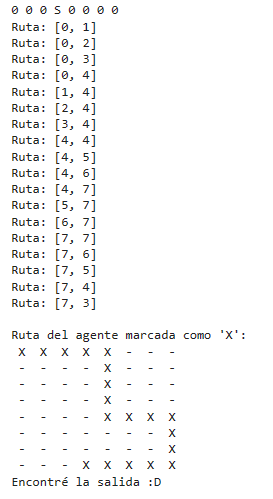
\includegraphics[scale = .6]{IMA/captuBFS.png}
    \caption{BFS}
    \label{fig:enter-label}
\end{figure}
\vspace{0.5cm}

\textbf{Ejemplo:}\\

Si elegimos el Laberinto 02, ambos algoritmos van a encontrar la salida. La diferencia sería:

\begin{itemize}
    \item \textbf{DFS:} Va a mostrar una ruta más larga pero válida.
    \item \textbf{BFS:} Va a garantizar la ruta más corta.
\end{itemize}

Entonces, la elección depende de nuestra prioridad, ya sea optimización o la exploración 
de diferentes caminos.